\documentclass[14pt]{extarticle}
\usepackage{siunitx}
\usepackage[a4 paper ,margin=2cm]{geometry}
\usepackage{enumitem}
\usepackage{graphicx}
\usepackage{titling}
\usepackage{float} % for [H] placement option
\usepackage{setspace}
\usepackage{gensymb}
\usepackage{mhchem} % For chemical equations
%\doublespacing
%\singlespacing

%\usepackage{graphicx}
%\usepackage{amssymb}
%\usepackage{relsize}
%\usepackage{amsthm}
%\interdisplaylinepenalty=2500
%\savesymbol{iint}
%\usepackage{txfonts}
%\restoresymbol{TXF}{iint}
%\usepackage{wasysym}
\usepackage{amsthm}
%\usepackage{iithtlc}
\usepackage{mathrsfs}
\usepackage{txfonts}
\usepackage{stfloats}
\usepackage{steinmetz}
\usepackage{bm}
\usepackage{cite}
\usepackage{cases}
\usepackage{subfig}
%\usepackage{xtab}
\usepackage{longtable}
\usepackage{tabularx}
\usepackage{multirow}
\usepackage{caption}
%\usepackage{algorithm}
%\usepackage{algpseudocode}
\usepackage{enumitem}
\usepackage{mathtools}
\usepackage{tikz}
\usepackage{circuitikz}
\usepackage{verbatim}
%\usepackage{textcomp}
\usepackage[breaklinks=true]{hyperref}
%\usepackage{stmaryrd}
\usepackage{tkz-euclide} % loads  TikZ and tkz-base
%\usetkzobj{all}
\usetikzlibrary{calc,math}
\usetikzlibrary{fadings}
\usepackage{listings}
    \usepackage{color}                                            %%
    \usepackage{array}                                            %%
    \usepackage{longtable}                                        %%
    \usepackage{calc}                                             %%
    \usepackage{multirow}                                         %%
    \usepackage{hhline}                                           %%
    \usepackage{ifthen}                                           %%
  %optionally (for landscape tables embedded in another document): %%
    \usepackage{lscape}     
\usepackage{multicol}
\usepackage{chngcntr}
%\usepackage{enumerate}

%\usepackage{wasysym}

\newtheorem{theorem}{Theorem}[section]
\newtheorem{problem}{Problem}
\newtheorem{proposition}{Proposition}[section]
\newtheorem{lemma}{Lemma}[section]
\newtheorem{corollary}[theorem]{Corollary}
\newtheorem{example}{Example}[section]
\newtheorem{definition}[problem]{Definition}
%\newcounter{MYtempeqncnt}
%\DeclareMathOperator*{\Res}{Res}
%\renewcommand{\baselinestretch}{2}
\renewcommand\thesection{\arabic{section}}
\renewcommand\thesubsection{\thesection.\arabic{subsection}}
\renewcommand\thesubsubsection{\thesubsection.\arabic{subsubsection}}



\setlength{\droptitle}{-6em}

\title{\textbf{\Huge XL - 2018}}
\author{EE25BTECH11049 - Sai Krishna Bakki}
\date{}

\begin{document}

\maketitle

\begin{flushleft}
\begin{center}   
\section*{General Aptitude (GA)}
\end{center}

\textbf{Q.1-Q.5 carry one mark each}


\begin{enumerate}
\item "Going by the \underline{\hspace{2cm}} that many hands make light work, the school \underline{\hspace{2cm}} involved all the students in the task."\\ [2ex]
The words that best fill the blanks in the above sentence are\\
\hfill(GATE XL 2018)\\
\begin{enumerate}
\begin{multicols}{2}

\item principle, principal
\item principal, principle
\item principle, principle
\item principal, principal
\end{multicols}
\end{enumerate}

\item "Her \underline{\hspace{2cm}} should not be confused with miserliness; she is ever willing to assist those in need."\\[2ex] The word that best fills the blank in the above sentence is\\
\hfill(GATE XL 2018)\\
\begin{enumerate}
\begin{multicols}{2}
\item cleanliness  
\item punctuality
\item frugality
\item greatness
\end{multicols}
\end{enumerate}

\item Seven machines take 7 minutes to make 7 identical toys. At the same rate, how many minutes would it take for 100 machines to make 100 toys?\\
\hfill(GATE XL 2018)\\
\begin{enumerate}
\begin{multicols}{2}
\item 1
\item 7
\item 100
\item 700
\end{multicols}
\end{enumerate}

\item A rectangle becomes a square when its length and breadth are reduced by 10 m and 5 m, respectively. During this process, the rectangle loses 650 m\textsuperscript{2} of area. What is the area of the original rectangle in square meters?\\
\hfill(GATE XL 2018)\\
\begin{enumerate}
\begin{multicols}{2}
\item 1125
\item 2250
\item 2924
\item 4500
\end{multicols}
\end{enumerate}

\item A number consists of two digits. The sum of the digits is 9. If 45 is subtracted from the number, its digits are interchanged. What is the number?\\
\hfill(GATE XL 2018)\\
\begin{enumerate}
\begin{multicols}{2}
\item 63
\item 72
\item 81
\item 90
\end{multicols}
\end{enumerate}
\textbf{Q.6-Q.10 carry two mark each}
  

\item For integers $a$, $b$ and $c$, what would be the minimum and maximum values respectively of $a+b+c$ if $\log |a| + \log |b| + \log |c| = 0$?\\
\hfill(GATE XL 2018)\\
\begin{enumerate}
\begin{multicols}{2}
\item -3 and 3
\item -1 and 1
\item -1 and 3
\item 1 and 3
\end{multicols}
\end{enumerate}

\item Given that $a$ and $b$ are integers and $a + a^2 b^3$ is odd, which one of the following statements is correct?\\
\hfill(GATE XL 2018)\\
\begin{enumerate}
\begin{multicols}{2}
\item $a$ and $b$ are both odd
\item $a$ and $b$ are both even
\item $a$ is even and $b$ is odd
\item $a$ is odd and $b$ is even
\end{multicols}
\end{enumerate}

\item From the time the front of a train enters a platform, it takes 25 seconds for the back of the train to leave the platform, while travelling at a constant speed of 54 km/h. At the same speed, it takes 14 seconds to pass a man running at 9 km/h in the same direction as the train. What is the length of the train and that of the platform in meters, respectively?\\
\hfill(GATE XL 2018)\\
\begin{enumerate}
\begin{multicols}{2}
\item 210 and 140
\item 162.5 and 187.5
\item 245 and 130
\item 175 and 200
\end{multicols}
\end{enumerate}

\item Which of the following functions describe the graph shown in the below figure?\\
\begin{figure}
    \centering
    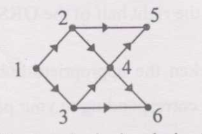
\includegraphics[width=0.5\columnwidth]{fig1.png}
    \caption{}
    \label{fig:q9}
\end{figure}

 \hfill(GATE XL 2018)\\
 \begin{enumerate}
 \begin{multicols}{2}
\item $y = ||x| + 1| - 2$
\item $y = ||x| - 1| - 1$
\item $y = ||x| + 1| - 1$
\item $y = ||x - 1| - 1|$
\end{multicols}
 \end{enumerate}

\item Consider the following three statements:  
    (i) Some roses are red.  
    (ii) All red flowers fade quickly.  
    (iii) Some roses fade quickly.  

Which of the following statements can be logically inferred from the above statements?
\hfill(GATE XL 2018)\\
\begin{enumerate}
\item If (i) is true and (ii) is false, then (iii) is false.
\item If (i) is true and (ii) is false, then (iii) is true.
\item If (i) and (ii) are true, then (iii) is true.
\item If (i) and (ii) are false, then (iii) is false.
    \end{enumerate}
\end{enumerate}
\begin{center}
    \textbf{END OF THE QUESTION PAPER}
\end{center}
\clearpage

\begin{center}
\section*{GATE 2018 – Chemistry (Compulsory) XL-P}
\end{center}
\textbf{Q.1-Q.5 carry one mark each}

\begin{enumerate}
\item For the complete combustion of graphite and diamond in oxygen individually, the standard enthalpy change ($\Delta H^\circ_{298}$) values are $-393.5$ kJ mol$^{-1}$ and $-395.4$ kJ mol$^{-1}$, respectively. Then, the $\Delta H^\circ_{298}$ for the conversion of graphite into diamond is \hfill (GATE XL 2018)\\
\begin{enumerate}
\begin{multicols}{2}
\item $+1.9$ kJ mol$^{-1}$
\item $-1.9$ kJ mol$^{-1}$
\item $+3.8$ kJ mol$^{-1}$
\item $-3.8$ kJ mol$^{-1}$
 \end{multicols} 
\end{enumerate}
\item For a 4s orbital of hydrogen atom, the magnetic quantum number ($m_l$) is\\
\hfill (GATE XL 2018)
\begin{enumerate}
\begin{multicols}{2}
\item 4
\item 3
\item 1
\item 0
\end{multicols}
\end{enumerate}

\item Hybridization of xenon in \ce{XeF2} is\\
\hfill (GATE XL 2018)\\
\begin{enumerate}
\begin{multicols}{2}
\item sp
\item sp$^2$
\item sp$^3$
\item sp$^3$d
\end{multicols}
\end{enumerate}

\item Two equivalents of \textbf{P} react with one equivalent of \textbf{Q} to produce a major product \textbf{R}. \hfill (GATE XL 2018)\\
\begin{figure}[H]
\centering
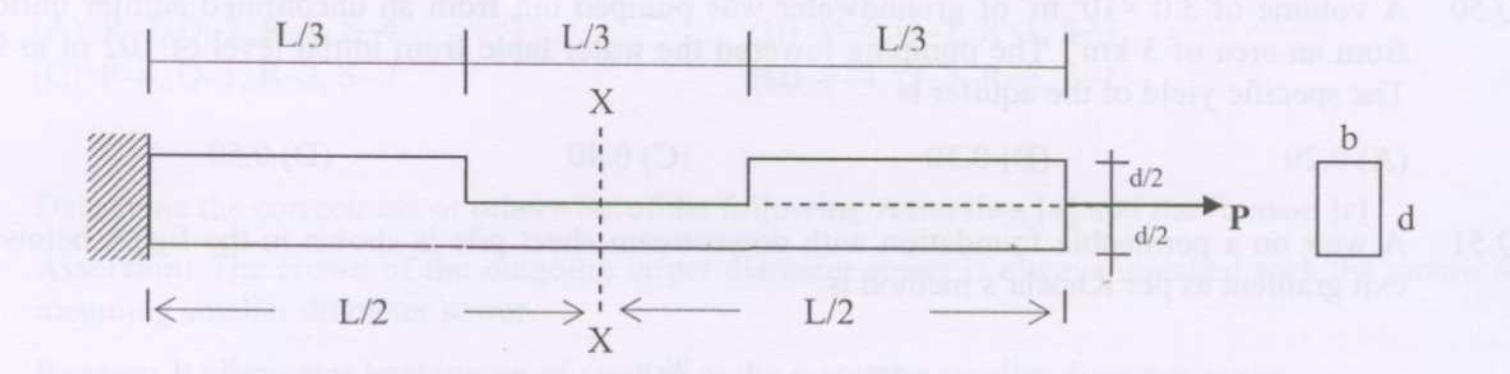
\includegraphics[width=1\columnwidth]{fig2.png}
\label{fig:q4}
\caption{}
\end{figure}
The number of double bonds present in the major product \textbf{R} is \underline{\hspace{3cm}}.

\item The total number of possible stereoisomers for the compound with the structural formula \ce{CH3CH(OH)CH=CHCH2CH3} is \underline{\hspace{3cm}}.\\
    \hfill (GATE XL 2018)\\

    \item Among B–H, C–H, N–H and Si–H bonds in \ce{BH3}, \ce{CH4}, \ce{NH3} and \ce{SiH4}, respectively, the polarity of the bond which is shown \textbf{INCORRECTLY} is\\
    \hfill (GATE XL 2018)\\
    \begin{enumerate}
    \begin{multicols}{2}
        \item B$^{\delta+}$–H$^{\delta-}$
        \item C$^{\delta-}$–H$^{\delta+}$
        \item N$^{\delta-}$–H$^{\delta+}$
        \item Si$^{\delta-}$–H$^{\delta+}$
        \end{multicols}
    \end{enumerate}

\item Among the following statements: \hfill (GATE XL 2018)\\
\begin{enumerate}[label=(\roman*)]
\item \ce{[NiCl4]^{2-}} (atomic number of Ni = 28) is diamagnetic
\item Ethylamine is a weaker Lewis base compared to pyridine
\item \ce{[NiCl2\{P(C6H5)3\}2]} has two geometrical isomers
\item Bond angle in \ce{H2O} is greater than that in \ce{H2S}
\end{enumerate}
The \textbf{CORRECT} one is:
\begin{enumerate}
\begin{multicols}{2}
\item (i)
\item (ii)
\item (iii)
\item (iv)
\end{multicols}
\end{enumerate}

\item In [\ce{Mn(H2O)6}]$^{2+}$ (atomic number of Mn = 25), the d–d transitions according to crystal field theory (CFT) are\\
\hfill (GATE XL 2018)\\
\begin{enumerate}
\item Laporte forbidden and spin forbidden
\item Laporte allowed and spin allowed
\item Laporte forbidden and spin allowed
\item Laporte allowed and spin forbidden
\end{enumerate}

\item The major product \textbf{M} in the reaction is\\
\hfill (GATE XL 2018)\\
\begin{figure}[H]
    \centering
    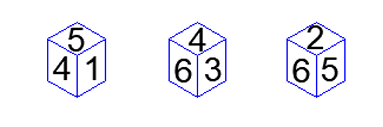
\includegraphics[width=0.9\columnwidth]{fig3.png}
    \caption{}
    \label{fig:q9}
\end{figure}
\clearpage   
\begin{enumerate}
\begin{multicols}{2}
\item 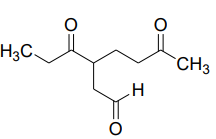
\includegraphics[width=0.5\columnwidth]{fig4.png}
\item 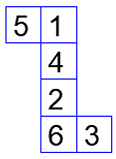
\includegraphics[width=0.5\columnwidth]{fig5.png}
\item 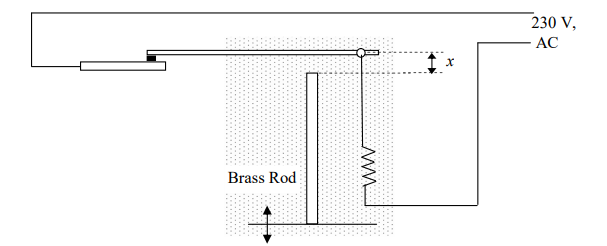
\includegraphics[width=0.5\columnwidth]{fig6.png}
\item 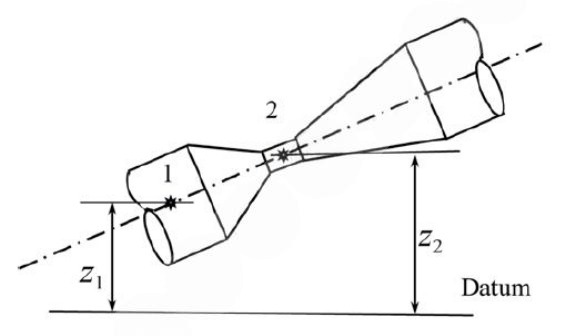
\includegraphics[width=0.5\columnwidth]{fig7.png}
\end{multicols}
\end{enumerate}

\item The two major products of the reaction are
\begin{figure}[H]
    \centering 
    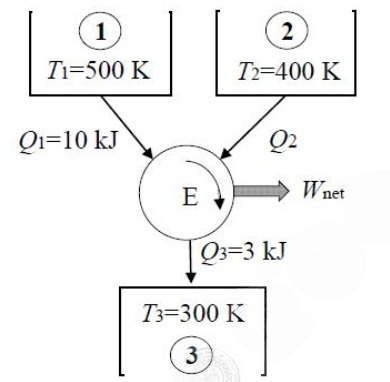
\includegraphics[width=0.8\columnwidth]{fig8.png}
    \caption{}
    \label{fig:q10} 
\end{figure}
\hfill (GATE XL 2018)\\
\begin{enumerate}
\item 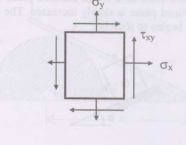
\includegraphics[width=0.2\columnwidth]{fig9.png} \textbf{and} \ce{CH2=CH2}
\item 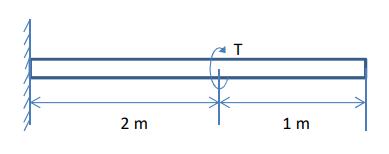
\includegraphics[width=0.2\columnwidth]{fig10.png}\textbf{and} \ce{N(CH3)2CH2CH3}
\item 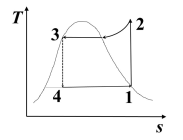
\includegraphics[width=0.2\columnwidth]{fig11.png}\textbf{and} \ce{N(CH3)2CH2CH3}
\item 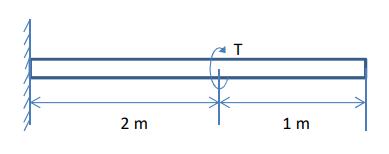
\includegraphics[width=0.2\columnwidth]{fig10.png}\textbf{and} \ce{HN(CH3)CH2CH3}
\end{enumerate}

\item The compound, which upon mono-nitration using a mixture of \ce{HNO3} and \ce{H2SO4}, does \textbf{NOT} give the meta-isomer as the major product, is \\
\hfill (GATE XL 2018)\\
\clearpage
\begin{enumerate}
\begin{multicols}{2}
\item 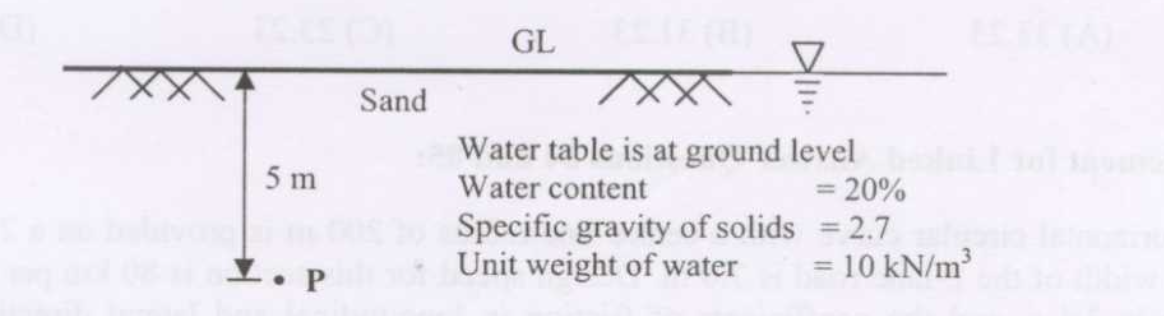
\includegraphics[width=0.2\columnwidth]{fig12.png}\\
\item 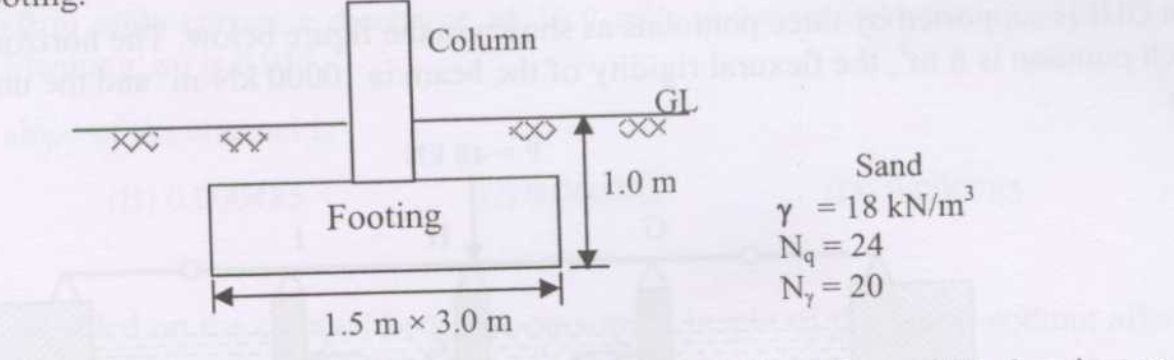
\includegraphics[width=0.2\columnwidth]{fig13.png}\\
\item 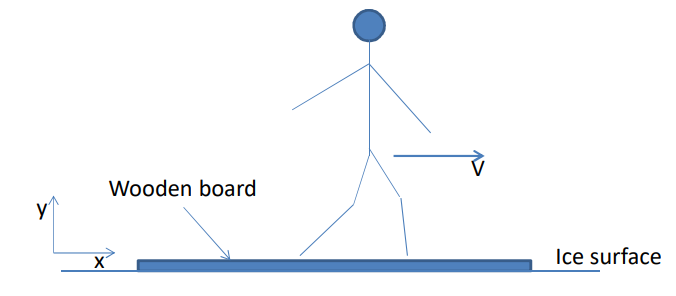
\includegraphics[width=0.2\columnwidth]{fig14.png}\\
\item 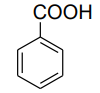
\includegraphics[width=0.2\columnwidth]{fig15.png}\\
\end{multicols}
\end{enumerate}

\item The standard reduction potential (E$^\circ$) for the conversion of \ce{Cr2O7^{2-}} to \ce{Cr^{3+}} at 25\,$^\circ$C in an aqueous solution of pH 3.0 is 1.33 V. The concentrations of \ce{Cr2O7^{2-}} and \ce{Cr^{3+}} are $1.0 \times 10^{-4}$ M and $1.0 \times 10^{-3}$ M, respectively. Then the potential of this half-cell reaction is \\
(\textbf{Given}: Faraday constant = 96500 C mol$^{-1}$, Gas constant R = 8.314 J K$^{-1}$ mol$^{-1}$)\\
    \hfill (GATE XL 2018)\\
\begin{enumerate}
\begin{multicols}{2}
\item 1.04 V
\item 0.94 V
\item 0.84 V
\item 0.74 V
\end{multicols}
\end{enumerate}

\item The solubility product (K$_\mathrm{sp}$) of \ce{Mg(OH)2} at 25\,$^\circ$C is $5.6 \times 10^{-11}$. Its solubility in water is $S \times 10^{-2}$ g/L, where the value of $S$ is \underline{\hspace{3cm}} (up to two decimal places). \hfill (GATE XL 2018)\\
(\textbf{Given}: Molecular weight of \ce{Mg(OH)2} = 58.3 g mol$^{-1}$)

\item The activation energy ($E_a$) values for two reactions carried out at 25\,$^\circ$C differ by 5.0 kJ mol$^{-1}$. If the pre-exponential factors (A$_1$ and A$_2$) for these two reactions are of the same magnitude, the ratio of rate constants ($k_1/k_2$) is \underline{\hspace{3cm}} (up to two decimal places). \hfill (GATE XL 2018)\\
(\textbf{Given}: Gas constant R = 8.314 J K$^{-1}$ mol$^{-1}$)

\item One mole of helium gas in an isolated system undergoes a reversible isothermal expansion at 25\,$^\circ$C from an initial volume of 2.0 liters to a final volume of 10.0 liters. The change in entropy ($\Delta S$) of the surroundings is \underline{\hspace{3cm}} J K$^{-1}$ (up to two decimal places). \hfill (GATE XL 2018)\\
(\textbf{Given}: Gas constant R = 8.314 J K$^{-1}$ mol$^{-1}$)

\end{enumerate}
\begin{center}
    \textbf{END OF THE QUESTION PAPER}
\end{center}
\clearpage

\begin{center}
    
\section*{GATE 2018 - Biochemistry-XL(Q)}
\noindent\textbf{Q. 1 -- Q. 10 carry one mark each. Q. 11 -- Q. 20 carry two marks each.}
\end{center}
\begin{enumerate}[leftmargin=*]

\item To which one of the following classes of enzymes does chymotrypsin belong?\\
\hfill(GATE XL 2018 )\\
\begin{enumerate}
\begin{multicols}{2}
\item Oxidoreductase
\item Hydrolyse
\item Transferase
\item somerase
\end{multicols}
\end{enumerate} 

\item The substrate saturation profile of an enzyme that follows Michaelis-Menten kinetics is depicted in the figure. What is the order of the reaction in the concentration range between 0.8 to 1.4 M?\\
\begin{figure}[H]
\centering
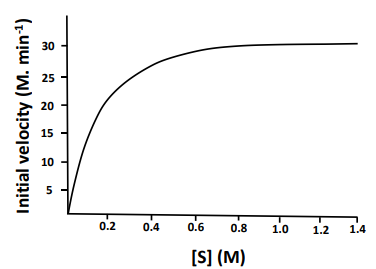
\includegraphics[width=0.6\columnwidth]{fig16.png}\\
\caption{}
\label{fig:q2}
\end{figure}
\hfill(GATE XL 2018)
\begin{enumerate}
\begin{multicols}{2}
\item Zero
\item Fraction
\item First
\item Second
\end{multicols}
\end{enumerate}

\item Which one of the following conformations of glucose is most stable?\\
\hfill(GATE XL 2018 )\\
\begin{enumerate}
\begin{multicols}{2}
\item Boat
\item Half Chair
\item Chair
\item Planar
\end{multicols}
\end{enumerate}

\item Which one of the following profiles represent the phenomenon of cooperativity?\\
\hfill(GATE XL 2018 )\\
\begin{enumerate}
\begin{multicols}{2}
\item 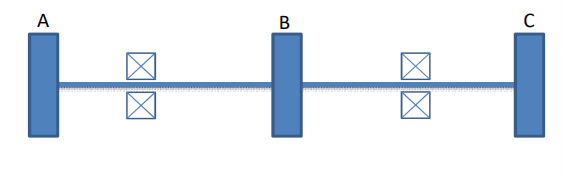
\includegraphics[width=0.4\columnwidth]{fig17.png}
\item 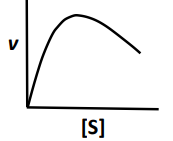
\includegraphics[width=0.4\columnwidth]{fig18.png}
\item 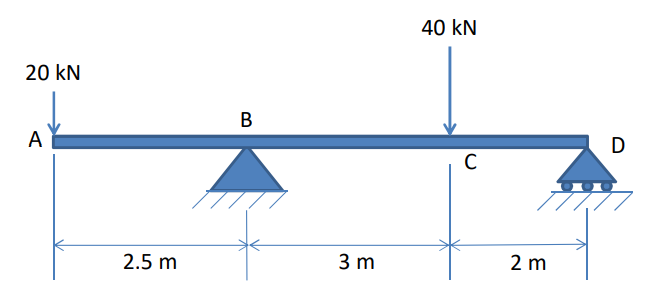
\includegraphics[width=0.4\columnwidth]{fig19.png}
\item 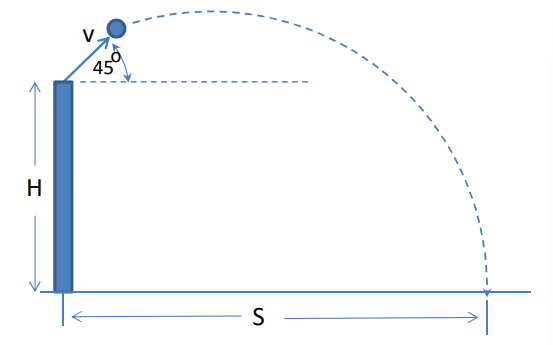
\includegraphics[width=0.4\columnwidth]{fig20.png}
\end{multicols}
\end{enumerate}

\item Which one of the following amino acids is responsible for the intrinsic fluorescence of proteins?\\
\hfill(GATE XL 2018 )\\
\begin{enumerate}
\begin{multicols}{2}
\item Pro
\item Meth
\item His
\item Trp
\end{multicols}
\end{enumerate}
\item The glycosylation of the proteins occurs in
\hfill(GATE XL 2018 )\\
\begin{enumerate}
\begin{multicols}{2}
    \item glyoxysomes
    \item lysosomes
    \item Golgi apparatus
    \item plasma membrane
\end{multicols}
\end{enumerate}


\item Which one of the following properties of the myeloma cells is used in the hybridoma technology to generate monoclonal antibody?
\hfill(GATE XL 2018 )\\
\begin{enumerate}
    \item lack of thymidylate synthase
    \item over-expression of hypoxanthine-guanine phosphoribosyl transferase
    \item over-expression of inosine 5$'$-monophosphate cyclohydrolase
    \item lack of hypoxanthine-guanine phosphoribosyl transferase
\end{enumerate}


\item The movement of protons through the FoF$_1$-ATPase during mitochondrial respiration is required for
\hfill(GATE XL 2018 )\\
\begin{enumerate}
    \item the increase in pH of mitochondrial matrix
    \item changing the conformation of FoF$_1$-ATPase to expel the ATP
    \item importing Pi from intermembrane space
    \item decreasing the affinity of ADP to FoF$_1$-ATPase
\end{enumerate}


\item The number of NADP$^+$ molecules required to completely oxidize one molecule of glucose to CO$_2$ through pentose phosphate pathway is \underline{\hspace{2cm}} (correct to integer number).
\hfill(GATE XL 2018 )\\


\item Measurement of the absorbance of a solution containing NADH in a path length of 1 cm cuvette at 340 nm shows the value of 0.31. The molar extinction coefficient of NADH is 6200 M$^{-1}$cm$^{-1}$. The concentration of NADH in the solution is \underline{\hspace{2cm}} $\mu$M (correct to integer number).\\[2ex]
\hfill(GATE XL 2018 )\\


\textbf{Q. 11 – Q. 20 carry two marks each.}

\item Among the reagents given below, which combination will \textbf{NOT} break the disulphide bonds in immunoglobulin molecules?\\[2ex]
\hfill(GATE XL 2018 )\\
\begin{enumerate}
\begin{multicols}{2}
\item Reduced glutathione
\item Dithiothritol
\item Sodium dodecyl sulphate
\item Methionine
\end{multicols}
\end{enumerate}

\begin{enumerate}
\begin{multicols}{2}
\item b,d
\item a,d
\item a,c
\item c,d
\end{multicols}
\end{enumerate}

\item Match the protein elution condition given in \textbf{Group I} with the appropriate chromatography matrices from \textbf{Group II}.

\begin{center}
\begin{tabular}{|c|p{8cm}|c|p{6cm}|}
\hline
\multicolumn{2}{|c|}{\textbf{Group I}} & \multicolumn{2}{c|}{\textbf{Group II}} \\
\hline
P & Increasing concentration of sodium chloride & i & Phenyl-Sepharose \\
Q & Increasing concentration of histidine & ii & Chromatofocusing \\
R & Decreasing concentration of ammonium sulphate & iii & DEAE-Sephacryl \\
S & Decreasing concentration of H$^+$ & iv & Ni-NTA \\
\hline
\end{tabular}
\end{center}

\hfill(GATE XL 2018 )\\
\begin{enumerate}
\begin{multicols}{2}
    \item P-iii; Q-iv; R-i; S-ii
    \item P-ii; Q-iv; R-i; S-iii
    \item P-i; Q-ii; R-iii; S-iv
    \item P-iv; Q-ii; R-iii; S-i
\end{multicols}
\end{enumerate}
\item Which one of the following is \textbf{NOT} a neurotransmitter?
\hfill(GATE XL 2018 )\\

\begin{enumerate}
\begin{multicols}{2}
    \item Adrenaline
    \item Glutamate
    \item Histamine
    \item Histidine
    \end{multicols}
\end{enumerate}
\clearpage

\item The type-II hypersensitivity reaction is mainly mediated by
\hfill(GATE XL 2018 )\\

\begin{enumerate}
\begin{multicols}{2} 
    \item IgE 
    \item IgM
    \item IgA
    \item T cells
    \end{multicols}
\end{enumerate}


\item Which reaction mechanism drives the conversion of 3-phosphoglyceraldehyde to 1,3-bisphosphoglycerate?
\hfill(GATE XL 2018 )\\

\begin{enumerate}
    \item Oxidation without anhydride bond formation
    \item Oxidation coupled with anhydride bond formation
    \item Substrate level phosphorylation
    \item Formation of carboxylate
\end{enumerate}


\item A polymerase reaction is carried out for 10 cycles in a volume of 1 mL with 5 molecules of template DNA. Assuming 100\% efficiency, the number of molecules of DNA present in 100 $\mu$L at the end of the reaction is \underline{\hspace{2cm}}.\\
\hfill(GATE XL 2018 )

\item The secondary structure topology diagram of a 400 amino acid long "Protein-X" is depicted in the figure. The start and end amino acid residue numbers of each $\alpha$-helix are marked. The percentage (correct to integer number) of residues forming $\alpha$-helix is \underline{\hspace{2cm}}.
\begin{figure}[H]
    \centering
    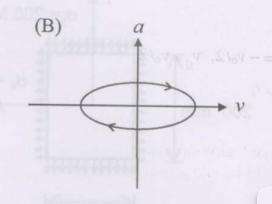
\includegraphics[width=0.9\columnwidth]{fig21.png}
    \caption{}
    \label{fig:q17}
\end{figure}

\hfill(GATE XL 2018 )


\item An enzyme follows Michaelis-Menten kinetics with substrate S. The fraction of the maximum velocity (V$_{max}$) will be observed with the substrate concentration [S] = 4$K_m$ is \underline{\hspace{2cm}}.(correct to decimal number)\\
\hfill(GATE XL 2018 )\\


\item The mass spectrum of benzoic acid will generate the fragment as a base peak (100\% relative abundance) of \textit{m/z} (mass to charge ratio) at \underline{\hspace{3cm}}
(correct to integer number)
\hfill(GATE XL 2018 )\\



\item The standard free energy ($\Delta G'$) values of reactions catalyzed by citrate lyase and citrate synthetase are $-670$ and $-8192$ cal/mol, respectively.

\[
\mathbf{Citrate}
\ \xrightleftharpoons[\text{}]{\text{\small Citrate lyase}}\
\mathbf{Acetate} + \mathbf{Oxaloacetate}
\quad \Delta G'_1 = -670 \ \text{cal/mol}
\]

\[
\mathbf{Acetyl\mbox{-}CoA} + \mathbf{Oxaloacetate} + H_2O
\ \xrightleftharpoons[\text{}]{\text{\small Citrate synthetase}}\
\mathbf{Citrate} + \mathrm{CoA}
\hspace{0.3cm} \Delta G'_2 = -8192 \ \text{cal/mol}
\]

The standard free energy (in cal/mol) of acetyl-CoA hydrolysis is \underline{\hspace{2cm}} (correct to integer number).
\hfill(GATE XL 2018 )\\

\begin{center}
\textbf{END OF THE QUESTION PAPER}
\end{center}

\end{enumerate}
\clearpage



\begin{center}   
\section*{GATE 2018 – Botany (XL-R)}
\noindent\textbf{Q. 1 -- Q. 10 carry one mark each. Q. 11 -- Q. 20 carry two marks each.}
\end{center}
\begin{enumerate}[leftmargin=*]
 \item Which of the following genera produces dimorphic seeds that help to broaden the time of germination in a variable habitat?\\
 \hfill(GATE XL 2018 )
    \begin{multicols}{2}
    \begin{enumerate}
        \item Xanthium
        \item Pisum
        \item Mangifera
        \item Linum
    \end{enumerate}
    \end{multicols}

    \item The genes for microRNA (miRNA) in plants are usually transcribed by\\
    \hfill(GATE XL 2018 )
    \begin{multicols}{2}
    \begin{enumerate}
        \item RNA polymerase I
        \item RNA polymerase II
        \item RNA polymerase III
        \item RNA polymerase IV
    \end{enumerate}
    \end{multicols}

    \item Which of the statements is \textbf{TRUE} for transposable elements Ac and Ds?\\
  \hfill(GATE XL 2018 ) 
    \begin{enumerate}
        \item Both Ac and Ds are autonomous because they encode their own transposase
        \item Both Ac and Ds are non-autonomous because they do not encode their own transposase
        \item Only Ac is autonomous because it encodes its own transposase
        \item Only Ds is autonomous because it encodes its own transposase
    \end{enumerate}
    

    \item Identify the \textbf{CORRECT} statement.\\
   \hfill(GATE XL 2018 )
    \begin{enumerate}
        \item Receptor-like kinases play role in gametophytic self-incompatibility in Brassicaceae
        \item Receptor-like kinases play role in sporophytic self-incompatibility in Solanaceae
        \item Ribonucleases play role in sporophytic self-incompatibility in Brassicaceae
        \item Ribonucleases play role in gametophytic self-incompatibility in Solanaceae
    \end{enumerate}
    

    \item Which of the following statements is \textbf{TRUE} for an ecotone?\\
   \hfill(GATE XL 2018 )
    \begin{enumerate}
        \item An ecotone is the synonym of an ecosystem
        \item An ecotone is an interface zone of two or more ecosystems
        \item An ecotone is a special feature of land biomes
        \item An ecotone is exclusively characterized by decreased biodiversity
    \end{enumerate}
    

    \item Acid rain with a pH of 4.0 is more acidic than the rain with a pH of 6.0 by\\
    \hfill(GATE XL 2018 )
    \begin{multicols}{2}
    \begin{enumerate}
        \item 2 times
        \item 10 times
        \item 100 times
        \item 1000 times
    \end{enumerate}
    \end{multicols}

    \item Which of the following plants produces Ylang-ylang oil?\\
    \hfill(GATE XL 2018 )
    \begin{multicols}{2}
    \begin{enumerate}
        \item Cananga odorata
        \item Carcum copticum
        \item Pandanus odoratissimus
        \item Pimenta racemosa
    \end{enumerate}
    \end{multicols}

    \item Identify the \textbf{INCORRECT} statement in connection with polar transport of auxin.\\
    \hfill(GATE XL 2018 )
    \begin{enumerate}
        \item The putative influx carrier AUX1 is a cytosolic protein
        \item Polar auxin transport in root tends to be both acropetal and basipetal in direction
        \item Naphthylphthalamic acid (NPA) is an inhibitor of polar auxin transport
        \item AUX1 and PIN1 proteins are located in the opposite ends of a cell for polar transport
    \end{enumerate}
     

    \item Which of the following stains is used to visualize callose under the microscope?\\
    \hfill(GATE XL 2018 )
    \begin{multicols}{2}
    \begin{enumerate}
        \item Alcian blue
        \item Aniline blue
        \item Toluidine blue
        \item Thymol blue
    \end{enumerate}
    \end{multicols}

    \item The coding sequence of a gene XLR18 has the single ORF of 783 bp. The approximate molecular weight of the XLR18 protein in kDa is \underline{\hspace{3cm}}.\\
    \hfill(GATE XL 2018 )

    \item Statements given below are either \textbf{TRUE (T)} or \textbf{FALSE (F)}. Select the \textbf{CORRECT} combination.  

    P. Mitosis occurs exclusively in diploid mother cell \\
    Q. Mitosis occurs both in diploid and haploid mother cells \\
    R. Meiosis occurs exclusively in diploid mother cell \\
    S. Meiosis occurs both in diploid and haploid mother cells\\
    \hfill(GATE XL 2018 )
    \begin{multicols}{2}
    \begin{enumerate}
        \item P-T, Q-F, R-T, S-F
        \item P-F, Q-T, R-F, S-T
        \item P-T, Q-F, R-F, S-T
        \item P-F, Q-T, R-T, S-F
    \end{enumerate}
    \end{multicols}

    \item You are asked to design a genetic construct for high-level expression of a gene encoding the therapeutic protein 18 (TP18) via plastid transformation. Select the \textbf{CORRECT} set of genetic elements for this construct.\\
 \hfill(GATE XL 2018 )   
    \begin{enumerate}
        \item Actin1 promoter $\rightarrow$ TP18 coding sequence $\rightarrow$ Actin1 transcription terminator
        \item Ubiquitin1 promoter $\rightarrow$ TP18 coding sequence $\rightarrow$ Ubiquitin1 transcription terminator
        \item rbcS promoter $\rightarrow$ TP18 coding sequence $\rightarrow$ rbcS transcription terminator
        \item rbcL promoter $\rightarrow$ TP18 coding sequence $\rightarrow$ rbcL transcription terminator
    \end{enumerate}
    

    \item Select the \textbf{CORRECT} combination of the following statements.  

    P. The cyclic electron transport chain involving PSI results in net production of both ATP and NADPH \\
    Q. The cyclic electron transport chain involving PSI results in net production of ATP \\
    R. Rubisco enzyme usually converts RuBP and CO$_2$ into 2-phosphoglycolate and 3-phosphoglycerate \\
    S. Rubisco enzyme usually converts RuBP and O$_2$ into 2-phosphoglycolate and 3-phosphoglycerate\\
    \hfill(GATE XL 2018 )
    \begin{multicols}{2}
    \begin{enumerate}
        \item P, Q
        \item R, S
        \item Q, S
        \item P, R
    \end{enumerate}
    \end{multicols}

\item Match the fruit characters with their families and representative plant species.\\
\hfill(GATE XL 2018 )

\begin{tabular}{p{4cm} p{4cm} p{6cm}}
\textbf{Fruit character} & \textbf{Family} & \textbf{Plant species} \\
P. Syconus & 1. Moraceae & i. \textit{Canavalia ensiformis} \\
Q. Capsule, opening by apical pores or valves & 2. Fabaceae & ii. \textit{Artabotrys odoratissimus} \\
R. Legume & 3. Papaveraceae & iii. \textit{Ficus religiosa} \\
S. An etaerio of drupe & 4. Annonaceae & iv. \textit{Papaver somniferum} \\
 & & v. \textit{Pistacia vera} \\
 & & vi. \textit{Citrus aurantium} \\
\end{tabular}

\begin{enumerate}
    \item P-2-iv, Q-3-ii, R-1-vi, S-4-v
    \item P-1-iii, Q-3-iv, R-2-i, S-4-ii
    \item P-3-i, Q-2-iii, R-4-ii, S-1-vi
    \item P-4-v, Q-1-ii, R-2-v, S-3-i
\end{enumerate}


\item  Select the \textbf{CORRECT} combination by matching the disease, affected plant and the causal organism.\\
\hfill(GATE XL 2018 )
\begin{tabular}{p{3.5cm} p{3cm} p{7cm}}
\textbf{Disease} & \textbf{Affected plant} & \textbf{Causal organism} \\
P. Black rot & 1. Corn & i. \textit{Fusarium oxysporum} f.sp. \textit{cubense} \\
Q. Loose smut & 2. Banana & ii. \textit{Acidovorax avenae} subsp. \textit{citrulli} \\
R. Panama wilt & 3. Watermelon & iii. \textit{Botryosphaeria obtusa} \\
S. Bacterial fruit blotch & 4. Apple & iv. \textit{Ustilago maydis} \\
 & & v. \textit{Plasmopara viticola} \\
 & & vi. \textit{Venturia inaequalis} \\
\end{tabular}

\begin{enumerate}
    \item P-2-v, Q-1-iv, R-3-iii, S-4-vi
    \item P-2-ii, Q-1-i, R-4-iii, S-3-i
    \item P-4-iii, Q-1-iv, R-2-i, S-3-ii
    \item P-4-vi, Q-1-iii, R-3-ii, S-2-v
\end{enumerate}

\item Select the \textbf{CORRECT} combination by matching \textbf{Group-I} with \textbf{Group-II}.\\
\hfill(GATE XL 2018 )
\begin{tabular}{p{5cm} p{6cm}}
\textbf{Group-I} & \textbf{Group-II} \\
P. Photorespiration & 1. Glutamate $\rightarrow$ 2-Oxoglutarate \\
Q. Respiration & 2. Acetyl-CoA $\rightarrow$ Malonyl-CoA \\
R. Amino acid degradation & 3. 2-Oxoglutarate $\rightarrow$ Succinyl-CoA \\
S. Fatty acid synthesis & 4. Glycine $\rightarrow$ Serine \\
\end{tabular}

\begin{enumerate}
    \item P-4, Q-2, R-3, S-4
    \item P-4, Q-1, R-4, S-1
    \item P-4, Q-3, R-1, S-2
    \item P-4, Q-2, R-3, S-2
\end{enumerate}

\item Match the plant alkaloids with their uses and source species.\\
\hfill(GATE XL 2018 )
\begin{tabular}{p{3cm} p{4cm} p{6cm}}
\textbf{Alkaloid} & \textbf{Use} & \textbf{Source species} \\
P. Codeine & 1. Stimulant & i. \textit{Hyoscyamus niger} \\
Q. Caffeine & 2. Analgesic & ii. \textit{Catharanthus roseus} \\
R. Scopolamine & 3. Antineoplastic & iii. \textit{Cola nitida} \\
S. Vinblastine & 4. Anticholinergic & iv. \textit{Papaver somniferum} \\
 & & v. \textit{Coptis japonica} \\
 & & vi. \textit{Senecio jacobaea} \\
\end{tabular}

\begin{enumerate}
    \item P-2-iv, Q-1-iii, R-4-i, S-3-ii
    \item P-4-iii, Q-2-v, R-1-vi, S-3-i
    \item P-2-v, Q-1-vi, R-3-iv, S-4-ii
    \item P-3-ii, Q-4-iii, R-1-iv, S-2-i
\end{enumerate}

    \item In garden pea, dwarf plants with terminal flowers are recessive to tall plants with axial flowers. A true-breeding tall plant with axial flowers was crossed with a true-breeding dwarf plant with terminal flowers. The resulting F1 plants were testcrossed, and the following progeny were obtained:  

    Tall plants with axial flowers = 320 \\
    Dwarf plants with terminal flowers = 318 \\
    Tall plants with terminal flowers = 79 \\
    Dwarf plants with axial flowers = 83  \\
    \hfill(GATE XL 2018 )\\
    The map distance between the genes for plant height and flower position is \underline{\hspace{3cm}} cM.

    \item Two true-breeding snapdragon (Antirrhinum majus) plants, one with red flowers and another with white flowers were crossed. The F1 plants were all with pink flowers. When the F1 plants were selfed, they produced three kinds of F2 plants with red, pink and white flowers in a 1:2:1 ratio. The probability that out of the five plants picked up randomly, two would be with pink flowers, two with white flowers and one with red flowers is \underline{\hspace{3cm}} \%.\\
    \hfill(GATE XL 2018 )
\end{enumerate}
\begin{center}
    \textbf{END OF THE QUESTION PAPER}
\end{center}
\clearpage

\begin{center}
 \textbf{\large{GATE 2018 — Microbiology (XL-S)}}\\[6pt]
 Q. 1 -- Q. 10 carry one mark each \& Q. 11 -- Q. 20 carry two marks each.\\[12pt]
\end{center}

\begin{enumerate}

\item David Baltimore’s classification of viruses is based on differences in\\
\hfill(GATE XL 2018 )\\
\begin{enumerate}
  \item host cell receptors used by viruses
  \item the pathways required to synthesize virus mRNA
  \item the modes of transmission of viruses
  \item the envelope proteins on the surface of viruses
\end{enumerate}

\item Which of the following immune system components can function as an opsonin?\\
\hfill(GATE XL 2018 )\\
\begin{enumerate}
\begin{multicols}{2}
  \item Antibodies
  \item T-cell receptors
  \item Histamines
  \item Interferons
  \end{multicols}
\end{enumerate}

\item The oral polio vaccine (OPV) consists of\\
\hfill(GATE XL 2018 )\\
\begin{enumerate}
\begin{multicols}{2}
  \item live attenuated virus
  \item killed virus
  \item viral toxin
  \item viral capsid subunit
  \end{multicols}
\end{enumerate}

\item Which of the following eukaryotic cellular components carries out intracellular degradation during autophagy?\\
\hfill(GATE XL 2018 )\\
\begin{enumerate}
\begin{multicols}{2}
  \item Nucleus
  \item Golgi bodies
  \item Ribosomes
  \item Lysosomes
  \end{multicols}
\end{enumerate}

\item Analysis of DNA sequences suggest that eukaryotic mitochondrial genomes primarily originated from\\
\hfill(GATE XL 2018 )\\
\begin{enumerate}
\begin{multicols}{2}
  \item fungi
  \item protozoa
  \item algae
  \item bacteria
  \end{multicols}
\end{enumerate}

\item Binomial nomenclature has \textbf{NOT} yet been adopted for\\
\hfill(GATE XL 2018 )\\
\begin{enumerate}
\begin{multicols}{2}
  \item bacteria
  \item fungi
  \item viruses
  \item protozoa
  \end{multicols}
\end{enumerate}

\item Which of the following is \textbf{NOT} an accepted method for sterilization?\\
\hfill(GATE XL 2018 )\\
\begin{enumerate}
\begin{multicols}{2}
  \item Autoclaving
  \item X-rays
  \item Gamma rays
  \item UV rays
  \end{multicols}
\end{enumerate}

\item The primary product of nitrogen fixation is\\
\hfill(GATE XL 2018 )\\
\begin{enumerate}
\begin{multicols}{2}
  \item N$_2$
  \item NH$_4^+$
  \item NO$_2^-$
  \item NO$_3^-$
  \end{multicols}
\end{enumerate}

\item In humans, the key stages in the life cycle of malarial parasites occur in\\
\hfill(GATE XL 2018 )\\
\begin{enumerate}
\begin{multicols}{2}
  \item red blood cells and the liver
  \item red blood cells and platelets
  \item red blood cells and the pancreas
  \item red blood cells and the gut
  \end{multicols}
\end{enumerate}

\item You have a 50 mg/mL stock solution of arginine. To prepare 1 liter of growth medium for an arginine auxotroph that requires 70 \textmu g/mL of arginine, the volume of this stock solution that should be added is \underline{\hspace{4cm}} mL (up to 1 decimal point).\\
\hfill(GATE XL 2018 )\\

\item Accumulating evidence suggest that Domain Archaea is more closely related to Domain Eukarya than to Domain Bacteria. Which of the following properties are shared between eukaryotes and archaea?
\begin{enumerate}
  \item Protein biogenesis
  \item Presence of sterol containing membranes
  \item Ribosomal subunit structures
  \item Adaptation to extreme environmental conditions
  \item Fatty acids with ester linkages in the cell membrane
\end{enumerate}
\hfill(GATE XL 2018 )\\
Options:
\begin{enumerate}
\begin{multicols}{2}
  \item (ii), (iii) and (v)
  \item (i), (ii), (iv), and (v)
  \item (i) and (iii)
  \item (iii) and (iv)
  \end{multicols}
\end{enumerate}

\item Match the antimicrobial agents in group I with their category/mode of action in group II.  

\begin{tabular}{|l|l|}
\hline
\textbf{Group I} & \textbf{Group II} \\ \hline
(i) Fluoroquinolones & (p) beta lactam antimicrobial \\
(ii) Amphotericin B & (q) inhibition of protein synthesis \\
(iii) Tetracycline & (r) inhibition of nucleic acid synthesis \\
(iv) Amoxicillin & (s) antifungal agent \\ \hline
\end{tabular}
\hfill(GATE XL 2018 )\\

\begin{enumerate}
\begin{multicols}{2}
  \item (i)-(q), (ii)-(s), (iii)-(r), (iv)-(p)
  \item (i)-(s), (ii)-(r), (iii)-(p), (iv)-(q)
  \item (i)-(r), (ii)-(s), (iii)-(q), (iv)-(p)
  \item (i)-(s), (ii)-(r), (iii)-(q), (iv)-(p)
  \end{multicols}
\end{enumerate}

\item Match the microorganisms to their predominant modes of transmission.  
\begin{tabular}{|l|l|}
\hline
\textbf{Microorganism} & \textbf{Mode of Transmission} \\ \hline
(i) \textit{Bordetella pertussis} & (p) Vector-borne \\
(ii) Dengue virus & (q) Blood-borne \\
(iii) \textit{Entamoeba histolytica} & (r) Droplet infection \\
(iv) Hepatitis B virus & (s) Contaminated food \\ \hline
\end{tabular}
\hfill(GATE XL 2018 )\\
\begin{enumerate}
\begin{multicols}{2}
  \item (i)-(r), (ii)-(p), (iii)-(s), (iv)-(q)
  \item (i)-(s), (ii)-(q), (iii)-(p), (iv)-(r)
  \item (i)-(q), (ii)-(p), (iii)-(s), (iv)-(r)
  \item (i)-(s), (ii)-(r), (iii)-(p), (iv)-(q)
  \end{multicols}
\end{enumerate}

\item Match the precursors/intermediates with the corresponding metabolic pathways.  \\
\begin{tabular}{|l|l|}
\hline
\textbf{Precursor/Intermediates} & \textbf{Metabolic pathway} \\ \hline
(i) Inosine monophosphate & (p) L-methionine biosynthesis \\
(ii) Ornithine & (q) L-tryptophan biosynthesis \\
(iii) Chorismate & (r) Purine biosynthesis \\
(iv) Homocysteine & (s) L-arginine biosynthesis \\ \hline
\end{tabular}
\hfill(GATE XL 2018 )\\
\begin{enumerate}
\begin{multicols}{2}
  \item (i)-(q), (ii)-(r), (iii)-(s), (iv)-(p)
  \item (i)-(p), (ii)-(r), (iii)-(s), (iv)-(q)
  \item (i)-(r), (ii)-(p), (iii)-(s), (iv)-(q)
  \item (i)-(r), (ii)-(s), (iii)-(q), (iv)-(p)
  \end{multicols}
\end{enumerate}

\item Match the scientists to their area of major contribution.  
\begin{center}
\begin{tabular}{|l|l|}
\hline
\textbf{Scientists} & \textbf{Area of major contribution} \\ \hline
(i) Antonie van Leeuwenhoek & (p) Taxonomy \\ 
(ii) Carl Linnaeus & (q) Antimicrobial agents \\ 
(iii) Sir Alexander Fleming & (r) Vaccination \\ 
(iv) Louis Pasteur & (s) Microscopy \\ \hline
\end{tabular}
\end{center}
\hfill(GATE XL 2018 )\\
\begin{enumerate}
\begin{multicols}{2}
  \item (i)-(s), (ii)-(q), (iii)-(p), (iv)-(r)
  \item (i)-(s), (ii)-(p), (iii)-(q), (iv)-(r)
  \item (i)-(p), (ii)-(s), (iii)-(r), (iv)-(q)
  \item (i)-(q), (ii)-(p), (iii)-(r), (iv)-(s)
  \end{multicols}
\end{enumerate}

\item Which of the following combinations would improve the resolution of a microscope?
\begin{enumerate}[label=(\roman*)]
  \item Increasing the half aperture angle of the objective lens
  \item Decreasing the wavelength of the illumination source
  \item Decreasing the numerical aperture of the objective lens
  \item Decreasing the refractive index of immersion medium
\end{enumerate}
\hfill(GATE XL 2018 )\\
Options:
\begin{enumerate}
\begin{multicols}{2}
  \item (i) and (ii)
  \item (ii) and (iii)
  \item (ii) and (iv)
  \item (i) and (iii)
  \end{multicols}
\end{enumerate}

\item Active transport involves the movement of a biomolecule against a concentration gradient across the cell membrane using metabolic energy. If the extracellular concentration of a biomolecule is 0.005 M and its intracellular concentration is 0.5 M, the least amount of energy that the cell would need to spend to transport this biomolecule from the outside to the inside of the cell is \underline{\hspace{4cm}} kcal/mol (up to 2 decimal points).\\
(Temperature $T = 298\,$K and universal gas constant $R = 1.98$ cal/mol$\cdot$K)
\hfill(GATE XL 2018 )\\

\item A continuous cell culture being carried out in a stirred tank reactor is described in terms of its cell mass concentration $X$ and substrate concentration $S$. The concentration of the substrate in the sterile feed stream is $S_F = 10$ g/L and yield coefficient $Y_{x/s} = 0.5$. The flow rates of the feed stream and the exit stream are equal ($F = 5$ mL/min) and constant. If the specific growth rate (h$^{-1}$) $\mu = \dfrac{0.3 S}{1+S}$, the steady state concentration of $S$ is \underline{\hspace{3cm}} g/L (up to 1 decimal point).\\
($V = 3\,$L given in original problem.)\\
\hfill(GATE XL 2018 )\\
\begin{figure}[H]
    \centering
    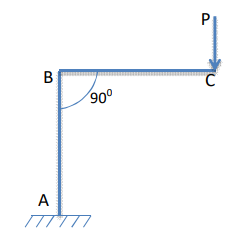
\includegraphics[width=0.5\columnwidth]{fig22.png}
    \caption{Caption}
    \label{fig:q18}
\end{figure}

\item The initial concentration of cells ($N_0$) growing unrestricted in a culture is $1.0\times10^{6}$ cells/mL. If the specific growth rate ($\mu$) of the cells is $0.1$ h$^{-1}$, the time required for the cell concentration to become $1.0\times10^{8}$ cells/mL is \underline{\hspace{3cm}} hours (up to 2 decimal points).
\hfill(GATE XL 2018 )\\

\item The following stoichiometric equation represents the conversion of glucose to lactic acid in a cell:
\hfill(GATE XL 2018 )\\
\[
\text{Glucose} + 2\;\text{Pi} + 2\;\text{ADP} \longrightarrow 2\;\text{Lactate} + 2\;\text{ATP} + 2\;\text{H}_2\text{O}
\]
If the free energy of conversion of glucose to lactic acid only is $\Delta G^0 = -47000$ cal/mol, the efficiency of energy transfer is \underline{\hspace{2.5cm}} \% (up to 1 decimal point).\\
\hfill(GATE XL 2018 )\\
($\Delta G^0$ for ATP hydrolysis is $-7.3$ kcal/mol.)

\end{enumerate}
\begin{center}
    \textbf{END OF THE QUESTION PAPER}
\end{center}
\clearpage

\begin{center}
\section*{GATE 2018 - Zoology (XL-T)}
\end{center}

\textbf{Q. 1 – Q. 10 carry one mark each.}\vspace{0.5em}


\begin{enumerate}
    \item Animals belonging to phylum Echinodermata are closer to chordates than other invertebrate phyla. Which ONE of the following reasons can account for this relatedness? \hfill(GATE XL 2018)\\
    \begin{multicols}{2}
    \begin{enumerate}
        \item Highly evolved nervous system
        \item Radially symmetric body plan
        \item Deuterostomic development
        \item Well-developed muscles
    \end{enumerate}
    \end{multicols}

    \item A zoologist recovered some tissue from preserved skin of a woolly mammoth. Further genetic analysis requires DNA isolation and increasing its amount. Which \textbf{ONE} of the following techniques would be most useful for increasing the amount of DNA?\hfill(GATE XL 2018)\\
    \begin{multicols}{2}
    \begin{enumerate}
        \item RFLP analysis
        \item Polymerase chain reaction (PCR)
        \item Electroporation
        \item Chromatography
    \end{enumerate}
    \end{multicols}

    \item In a chemical reaction where the substrate and product are in equilibrium in solution, what will occur if an enzyme is added? \hfill(GATE XL 2018)\\
    \begin{enumerate}
        \item The equilibrium of the reaction will not change.
        \item There will be a decrease in product formed.
        \item Additional substrate will be formed.
        \item The free energy of the system will change.
    \end{enumerate}

    \item Tay-Sachs disease is a human genetic disorder that is associated with defects in which \text{ONE} of the following cellular organelles? 
    \hfill(GATE XL 2018)\\
    \begin{multicols}{2}
    \begin{enumerate}
        \item Endoplasmic reticulum
        \item Mitochondria
        \item Golgi apparatus
        \item Lysosome
    \end{enumerate}
    \end{multicols}

    \item Increase in the existent population of grey peppered moth, \textit{Biston betularia}, during industrial revolution in Britain is an example of which ONE of the following evolutionary processes? \hfill(GATE XL 2018)\\
    \begin{multicols}{2}
    \begin{enumerate}
        \item Neutral selection
        \item Disruptive selection
        \item Directional selection
        \item Stabilizing selection
    \end{enumerate}
    \end{multicols}
    

    \item Which ONE of the following is NOT a characteristic of a cancer cell?\\
    \hfill(GATE XL 2018)\\
    \begin{multicols}{2}
    \begin{enumerate}
        \item Increase in cell motility
        \item Loss of contact inhibition
        \item Decrease in apoptosis
        \item Uncontrolled meiosis
    \end{enumerate}
    \end{multicols}

    \item Cardiac and cerebral tissues are derived from the following germ layers respectively \hfill(GATE XL 2018)\\
    \begin{multicols}{2}
    \begin{enumerate}
        \item Ectoderm and mesoderm
        \item Mesoderm and ectoderm
        \item Mesoderm and endoderm
        \item Endoderm and ectoderm
    \end{enumerate}
    \end{multicols}

    \item An animal’s ability to escape from a predator by using the explored knowledge of home area is an example of \hfill(GATE XL 2018)\\
    \begin{multicols}{2}
    \begin{enumerate}
        \item Latent learning
        \item Insight learning
        \item Mimicry
        \item Imprinting
    \end{enumerate}
    \end{multicols}

    \item Bowman's capsules are present in which ONE of the following organs/tissues? \hfill(GATE XL 2018)\\
    \begin{multicols}{2}
    \begin{enumerate}
        \item Renal cortex
        \item Urinary bladder
        \item Renal medulla
        \item Ureter
    \end{enumerate}
    \end{multicols}

    \item Which \textbf{ONE} of the following is the primary function of lung surfactants?\\
    \hfill(GATE XL 2018)\\
    \begin{enumerate}
        \item Remove dust particles from bronchi
        \item Provide immunity to respiratory tract
        \item Prevent alveoli from collapsing by decreasing surface tension
        \item Aid in carbon dioxide exchange
    \end{enumerate}

    \item Match the disorders/diseases listed in Column I to their respective causative agents listed in Column II. \hfill(GATE XL 2018)\\
\begin{tabular}{p{6cm} p{6cm}}
\textbf{Column I} & \textbf{Column II} \\
I) African tick bite fever & i) \textit{Trypanosoma gambiense} \\
II) Yellow fever & ii) Zika virus \\
III) Microcephaly & iii) \textit{Rickettsia sp.} \\
IV) Sleeping sickness & iv) Flavivirus \\
\end{tabular}

\begin{multicols}{2}
 \begin{enumerate}
        \item I-iv, II-iii, III-ii, IV-i
        \item I-iii, II-iv, III-ii, IV-i
        \item I-iii, II-iv, III-i, IV-ii
        \item I-iii, II-i, III-iv, IV-ii
    \end{enumerate}
    \end{multicols}

    \item Glucose monomers are joined together by glycosidic linkages to form a cellulose polymer. During this process, changes in the free energy, total energy, and entropy respectively are represented correctly by which \textbf{ONE} of the following options? \hfill(GATE XL 2018)\\
    \begin{multicols}{2}
    \begin{enumerate}
        \item +$\Delta$G, +$\Delta$H, +$\Delta$S
        \item +$\Delta$G, -$\Delta$H, -$\Delta$S
        \item -$\Delta$G, +$\Delta$H, +$\Delta$S
        \item +$\Delta$G, +$\Delta$H, -$\Delta$S
    \end{enumerate}
    \end{multicols}

\item In \textit{Drosophila melanogaster}, a mutation in \textit{Ultrabithorax} which defines the third segment of the thorax or T3 leads to development of four winged flies, as the halteres develop into a 
second pair of wings. Which \textbf{ONE} of the following phenotypes in fly will result from 
overexpression of Ultrabithorax in the second thoracic segment? 
    \hfill(GATE XL 2018)\\
    \begin{multicols}{2}
    \begin{enumerate}
        \item Four winged flies
        \item Two wings and two halteres flies
        \item Flies with four halteres
        \item Flies with two halteres
    \end{enumerate}
    \end{multicols}

    \item Which \textbf{ONE} of the following is \textbf{TRUE} in case of respiratory acidosis? \hfill(GATE XL 2018)\\
    \begin{enumerate}
        \item Increased rate of ventilation is a cause
        \item Blood pH more than 7
        \item Increased levels of carbon dioxide in blood
        \item Compensated by reducing bicarbonate in plasma
    \end{enumerate}

    \item Match the proteins/molecules listed in Column I with the cellular location in Column II. \hfill(GATE XL 2018)\\
\begin{tabular}{p{6cm} p{6cm}}
\textbf{Column I} & \textbf{Column II} \\
I) Galactosyl transferase & (i) Vesicles \\
II) Cytochrome oxidase & (ii) Cytosol \\
III) Clathrin & (iii) Golgi complex \\
IV) Tubulin & (iv) Mitochondria \\
\end{tabular}
    \begin{multicols}{2}
    \begin{enumerate}
        \item I-ii; II-iii; III-i; IV-iv
        \item I-iii; II-iv; III-i; IV-ii
        \item I-iii; II-iv; III-ii; IV-i
        \item I-iv; II-iii; III-ii; IV-i
    \end{enumerate}
    \end{multicols}

    \item In an experiment, nucleus from  \textit{Drosophila} oocyte  was transplanted into the anterior part of another oocyte, at a region opposite to the existing nucleus. Which \textbf{ONE} of the 
    following phenotypes will the developing egg show?\\  \hfill(GATE XL 2018)\\
    \begin{enumerate}
        \item A ventralized egg with no dorsal appendages
        \item A dorsalized egg with two dorsal appendages
        \item A ventralized egg with two dorsal appendages
        \item A dorsalized egg with four dorsal appendages
    \end{enumerate}

    \item Match the organisms in Column I with features in Column II.\\ 
    \hfill(GATE XL 2018)\\
\begin{tabular}{p{6cm} p{6cm}}
\textbf{Column I} & \textbf{Column II} \\
I) Tapeworm & (i) Bioluminescence \\
II) Jellyfish & (ii) Viviparous \\
III) Trichinella & (iii) Lateral heart \\
IV) Earthworm & (iv) Microvilli on the body surface \\
\end{tabular}
    \begin{multicols}{2}
    \begin{enumerate}
        \item I-iii; II-i; III-iv; IV-ii
        \item I-ii; II-iv; III-i; IV-iii
        \item I-iv; II-i; III-ii; IV-iii
        \item I-iv; II-iii; III-ii; IV-i
    \end{enumerate}
    \end{multicols}

    \item Which \textbf{ONE} of the following statements is \textbf{NOT} part of the classical Darwinian theory of evolution by natural selection? \hfill(GATE XL 2018)\\
    \begin{enumerate}
        \item A trait constantly used will get inherited
        \item Phenotypic variations exist in a population
        \item Fittest individuals are more likely to survive
        \item Each population acquires variations randomly
    \end{enumerate}

\item A population of rabbitswas determined to have a birth rate of 200 and mortality rate of 50 per year. If the initial population size is 4000 individuals, after 2 years of non-interfered breeding the final population size will be \underline{\hspace{3cm}} 
\hfill(GATE XL 2018)\\

\item In a population in Hardy-Weinberg equilibrium m, the frequency of occurrence of a disorder caused by recessive allele (q) is 1 in 1100. The frequency of heterozygotes in the population will be  \underline{\hspace{3cm}} \\
\hfill(GATE XL 2018)

\end{enumerate}
\begin{center}
    \textbf{END OF THE QUESTION PAPER}
\end{center}
\clearpage


\begin{center}
 \section*{GATE 2018 - Food Technology (XL-U)}
 \end{center}
 
\textbf{Q.~1 -- Q.~10 carry one mark each. Q.~11 -- Q.~20 carry two marks each.}\\

\begin{enumerate}
\item Which of the following is an oil soluble pigment present in fruits and vegetables?\\
\hfill(GATE XL 2018 )\\
\begin{enumerate}
\begin{multicols}{2}
    \item Flavonoids
    \item Carotenoids
    \item Anthocyanins
    \item Tannins
    \end{multicols}
\end{enumerate}

\item Which of the following represent the group of saturated fatty acids?\\
\hfill(GATE XL 2018 )\\
\begin{enumerate}
\begin{multicols}{2}
    \item Lauric, Myristic, Arachidic
    \item Palmitic, Linoleic, Linolenic
    \item Capric, Stearic \& Oleic
    \item Behenic, Caprylic, Arachidonic
    \end{multicols}
\end{enumerate}

\item The anti-nutritional factor present in fava bean is\\
\hfill(GATE XL 2018 )\\
\begin{enumerate}
\begin{multicols}{2}
    \item Gossypol
    \item Curcine
    \item Vicine
    \item Cyanogen
    \end{multicols}
\end{enumerate}

\item Which of the following is a Gram positive bacteria?\\
\hfill(GATE XL 2018 )\\
\begin{enumerate}
\begin{multicols}{2}
    \item Listeria monocytogenes
    \item Proteus vulgaris
    \item Salmonella typhi
    \item Shigella dysenteriae
    \end{multicols}
\end{enumerate}

\item Irradiation carried out to reduce viable non-spore forming pathogenic bacteria using a dose between 3 to 10 kGy is\\
\hfill(GATE XL 2018 )\\
\begin{enumerate}
\begin{multicols}{2}
    \item Radurization
    \item Thermoradiation
    \item Radappertization
    \item Radicidation
    \end{multicols}
\end{enumerate}

\item Identify the correct statement related to the viscosity of Newtonian fluids from the following.\\
\hfill(GATE XL 2018 )\\

\begin{enumerate}
    \item It is not influenced by temperature
    \item It increases with shearing rate
    \item It decreases with shearing rate
    \item It is not influenced by shearing rate
\end{enumerate}

\item Adult male Wistar rats were fed with a protein based diet. Total 150 g of protein was ingested per animal. If the average weight increased from 110 g to 350 g after the end of experiment, the Protein efficiency ratio of the given protein would be \underline{\hspace{2cm}} (up to two decimal points).\\
\hfill(GATE XL 2018 )\\


\item The initial moisture content of a food on wet basis is 50.76\%. Its moisture content (\%) on dry basis is \underline{\hspace{2cm}} (up to two decimal points).\\
\hfill(GATE XL 2018 )\\

\item The oxygen transmission rate through a $2.54\times 10^{-3}$ cm thick low density polyethylene film with air on one side and inert gas on the other side is $3.5\times 10^{-6}$ mL cm$^{-2}$ s$^{-1}$. Oxygen partial pressure difference across the film is 0.21 atm. The permeability coefficient of the film to oxygen is \underline{\hspace{2cm}} $\times 10^{-11}$ mL (STP) cm cm$^{-2}$ s$^{-1}$ (cm Hg)$^{-1}$.\\
\hfill(GATE XL 2018 )\\

\item Ambient air at $30^\circ$C dry bulb temperature and 80\% relative humidity was heated to a dry bulb temperature of $80^\circ$C in a heat exchanger by indirect heating. The amount of moisture gain (g kg$^{-1}$ dry air) during the process would be \underline{\hspace{2cm}}.\\
\hfill(GATE XL 2018 )\\

\item Match the commodity in Group I with the bioactive constituent in Group II:
\[
\begin{array}{ll}
\textbf{Group I} & \textbf{Group II} \\
P. \ \text{Ginger} & 1. \ \text{Lutein} \\
Q. \ \text{Green tea} & 2. \ \text{Gingerol} \\
R. \ \text{Spinach} & 3. \ \text{Curcumin} \\
S. \ \text{Turmeric} & 4. \ \text{Epigallocatechin gallate} \\
\end{array}
\]
\hfill(GATE XL 2018 )\\
\begin{enumerate}
\begin{multicols}{2}
    \item P-1, Q-2, R-3, S-4
    \item P-2, Q-4, R-1, S-3
    \item P-4, Q-1, R-3, S-2
    \item P-2, Q-3, R-1, S-4
    \end{multicols}
\end{enumerate}

\item Match the process operation in Group I with the separated constituent in Group II:
\[
\begin{array}{ll}
\textbf{Group I} & \textbf{Group II} \\
P. \ \text{Extraction} & 1. \ \text{Phospholipids} \\
Q. \ \text{Degumming} & 2. \ \text{Free fatty acids} \\
R. \ \text{Neutralization} & 3. \ \text{Pigments} \\
S. \ \text{Bleaching} & 4. \ \text{Crude oil} \\
\end{array}
\]
\hfill(GATE XL 2018 )\\
\begin{enumerate}
\begin{multicols}{2}
    \item P-3, Q-2, R-4, S-1
    \item P-4, Q-3, R-1, S-2
    \item P-4, Q-1, R-2, S-3
    \item P-4, Q-1, R-3, S-2
    \end{multicols}
\end{enumerate}

\item Match the spoilage symptom in Group I with the causative microorganism in Group II:
\[
\begin{array}{ll}
\textbf{Group I} & \textbf{Group II} \\
P. \ \text{Green rot of eggs} & 1. \ \text{Micrococcus spp.} \\
Q. \ \text{Putrid swell in canned fish} & 2. \ \text{Serretia marcescens} \\
R. \ \text{Red bread} & 3. \ \text{Pseudomonas fluorescens} \\
S. \ \text{Yellow discoloration of meat} & 4. \ \text{Clostridium sporogens} \\
\end{array}
\]
\hfill(GATE XL 2018 )\\
\begin{enumerate}
\begin{multicols}{2}
    \item P-4, Q-3, R-2, S-1
    \item P-2, Q-1, R-4, S-3
    \item P-3, Q-4, R-2, S-1
    \item P-1, Q-4, R-3, S-2
    \end{multicols}
\end{enumerate}

\item Match the fermented product in Group I with the base material in Group II:
\[
\begin{array}{ll}
\textbf{Group I} & \textbf{Group II} \\
P. \ \text{Sake} & 1. \ \text{Milk} \\
Q. \ \text{Chhurpi} & 2. \ \text{Cabbage} \\
R. \ \text{Natto} & 3. \ \text{Rice} \\
S. \ \text{Sauerkraut} & 4. \ \text{Soybean} \\
\end{array}
\]
\hfill(GATE XL 2018 )\\

\begin{enumerate}
\begin{multicols}{2}
    \item P-3, Q-1, R-4, S-2
    \item P-1, Q-3, R-4, S-2
    \item P-4, Q-1, R-3, S-2
    \item P-2, Q-4, R-1, S-3
    \end{multicols}
\end{enumerate}

\item Match the operation in Group I with the process in Group II:
\[
\begin{array}{ll}
\textbf{Group I} & \textbf{Group II} \\
P. \ \text{Cleaning} & 1. \ \text{Quality separation} \\
Q. \ \text{Grading} & 2. \ \text{Clarification} \\
R. \ \text{Size reduction} & 3. \ \text{Screening} \\
S. \ \text{Filtration} & 4. \ \text{Comminution} \\
\end{array}
\]
\hfill(GATE XL 2018 )\\

\begin{enumerate}
\begin{multicols}{2}
    \item P-1, Q-3, R-4, S-2
    \item P-4, Q-1, R-3, S-2
    \item P-2, Q-4, R-1, S-3
    \item P-3, Q-1, R-4, S-2
    \end{multicols}
\end{enumerate}

\item Out of 7 principles of HACCP system, 4 are listed below. Arrange these principles in the order in which they are applied:
(P) Conduct a hazard analysis \\
(Q) Establish monitoring process \\
(R) Establish critical limit \\
(S) Establish record keeping and documentation process\\
\hfill(GATE XL 2018 )\\

\begin{enumerate}
\begin{multicols}{2}
    \item P, R, Q, S
    \item Q, R, P, S
    \item P, Q, R, S
    \item R, S, P, Q
    \end{multicols}
\end{enumerate}

\item Identify an example of a classical diffusional mass transfer process without involving heat, among the following.\\
\hfill(GATE XL 2018 )\\

\begin{enumerate}
\begin{multicols}{2}
    \item Drying of food grains
    \item Carbonation of beverages
    \item Distillation of alcohol
    \item Concentration of fruit juice
    \end{multicols}
\end{enumerate}

\item For an enzyme catalyzed reaction $S \rightarrow P$, the kinetic parameters are: \\
$[S] = 40\ \mu$M, $V_0 = 9.6\ \mu$M s$^{-1}$, and $V_{\max} = 12.0\ \mu$M s$^{-1}$. \\
The $K_m$ of the enzyme in $\mu$M will be \underline{\hspace{2cm}} (up to one decimal point).\\
\hfill(GATE XL 2018 )\\


\item A microbial sample taken at 10 AM contained $1\times 10^5$ CFU/mL. The count reached to $1\times 10^{10}$ CFU/mL at 8 PM of the same day. The growth rate (h$^{-1}$) of the microorganism would be \underline{\hspace{2cm}} (up to two decimal points).\\
\hfill(GATE XL 2018 )\\

\item The rate of heat transfer per unit area from a metal plate is 1000 W m$^{-2}$. The surface temperature of the plate is $120^\circ$C and ambient temperature is $20^\circ$C. The convective heat transfer coefficient (W m$^{-2}$~$^\circ$C$^{-1}$) using the Newton's law of cooling will be \underline{\hspace{2cm}}.
\hfill(GATE XL 2018 )\\

\end{enumerate}
\begin{center}
    \textbf{END OF THE QUESTION PAPER}
\end{center}

\end{flushleft}
\end{document}